\documentclass[12pt,letterpaper]{article}

%Langue et caractères spéciaux
\usepackage[french]{babel}
\usepackage[utf8]{inputenc}
%Marges
\usepackage[top=2cm, bottom=2cm, left=2cm, right=2cm]{geometry}
\setlength\parindent{0pt}
%Graphiques
\usepackage{graphicx}
\usepackage{booktabs}


%%%%%%%%%%%%
% Document %
%%%%%%%%%%%%
\begin{document}

%%%%%%%%%%%%%%
% Page titre %
%%%%%%%%%%%%%%
\begin{titlepage}
\begin{center}


\includegraphics[width=0.25\textwidth]{../poly.png}~\\[1cm]

\textsc{\huge École Polytechnique de Montréal}\\[1cm]

\rule{0.5\linewidth}{0.5mm} \\[0.4cm]
{\LARGE Travail pratique 1}\\[0.6cm]

{\large INF4410}\\[0.2cm]
{\large \textbf{Systèmes répartis et infonuagique}}\\[0.4cm]

\rule{0.5\linewidth}{0.5mm} \\[1cm]

{\large par}\\[0.6cm]
\begin{Large}
  \begin{tabular}{r l}
    Samuel \textsc{Lavoie} & 1688635\\[0.4cm]
    Samuel \textsc{Rondeau} & 1723869\\[0.4cm]
  \end{tabular}
\end{Large}

\vfill

{\large \today}\\[0.5cm]
{\large Département de génie informatique et génie logiciel}\\[0.2cm]
{\large École Polytechnique de Montréal}

\end{center}
\end{titlepage}


%%%%%%%%%%%%
% Partie 1 %
%%%%%%%%%%%%
\section*{Partie 1}
\hrule
\vspace{1em}

%%%%%%%
% 1.1 %
%%%%%%%
\subsection*{Question 1}
Nous pouvons observer qu'en ce qui à trait à la fonction normale, le temps pour appeler une fonction ne dépend pas de la taille des paramètres.
Le temps demeure approximativement constant en fonction de la taille des paramètres.\\
\\
Par contre, pour ce qui est des deux autre fonctions (locale et distante), le temps croît exponentiellement avec la taille des paramètres.
Ceci est dû au fait que lors de l'appel RMI, les données doivent être sérialisées, écrites dans un socket, lues du socket et désérialisées.\\
\\
Pour ce qui est de la fonction distante, celle-ci doit en plus envoyer les informations à un serveur distant.
Ceci entraîne donc des délais de latence additionnels.

\paragraph{Avantages Java RMI :}
Très simple d'utilisation.
Il est possible d'envoyer des objets sur un socket sans ce soucier des détails d'implémentation.
Ceci permet donc un développement plus rapide.

\paragraph{Désavantages Java RMI :}
Il y a des coûts additionnels à l'abstraction.
Le programmeur ne contrôle pas les détails d'implémentation.
Il peut donc être difficile d'effectuer des actions qui sortent de celles prescrites pas la librairie.

\begin{table}[h]
  \centering
  \begin{tabular}{rrrr}
    \toprule
    \textbf{x ($octets$)} & \textbf{Appel normal ($ns$)} & \textbf{RMI local ($ns$)} & \textbf{RMI distant ($ns$)} \\ \hline
            $10$ & $2~845$ &   $1~200~850$ &   $1~034~526$ \\
           $100$ & $2~959$ &   $1~286~645$ &   $2~041~399$ \\
         $1~000$ & $2~949$ &   $1~285~203$ &   $2~088~678$ \\
        $10~000$ & $3~062$ &   $3~585~502$ &   $3~202~298$ \\
       $100~000$ & $2~920$ &   $6~659~594$ &  $11~550~960$ \\
     $1~000~000$ & $3~073$ &  $15~932~887$ &  $90~006~724$ \\
    $10~000~000$ & $3~139$ & $141~864~770$ & $887~660~336$ \\
    \bottomrule
  \end{tabular}
  \caption{Temps de réponse des 3 appels en fonction de la taille des paramètres.}
  \label{tab:temps}
\end{table}

\begin{figure}[h]
  \centering
  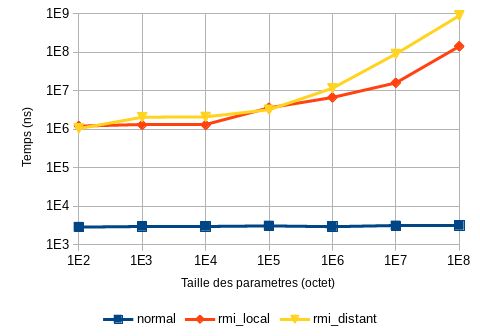
\includegraphics{graph.png}
  \caption{Temps de réponse des 3 appels en fonction de la taille des paramètres.}
  \label{fig:temps}
\end{figure}

%%%%%%%
% 1.2 %
%%%%%%%
\subsection*{Question 2}
\begin{enumerate}
  \item La classe \texttt{Server} implémente l'interface \texttt{ServerInterface}, qui dérive de l'interface \\
        \texttt{java.rmi.Remote}. Ainsi, la classe \texttt{Server} implémente un \textbf{registre RMI}.
  \item Le serveur distant (\texttt{Server}) est initialisé avec la méthode \texttt{Server.run()}.
  \item Le serveur local (\texttt{Server}) est initialisé avec la méthode \texttt{Server.run()}.
  \item Le client crée un nouvel objet \texttt{FakeServer} pour l'appel normal.
  \item Le client se connecte au \textbf{serveur local} pour l'appel RMI local avec la méthode \\
        \texttt{Client.loadServerStub()}.
  \item Le client se connecte au \textbf{serveur distant} pour l'appel RMI distant avec la méthode \\
        \texttt{Client.loadServerStub()}.
  \item Le code client est executé avec la méthode \texttt{Client.run()}.
  \item Le client exécute l'\textbf{appel normal} avec la méthode \texttt{Client.appelNormal()}.
  \item Le client lance l'exécution locale (par \texttt{FakeServer}) d'un calcul avec la méthode \\
        \texttt{FakeServer.execute()}.
  \item Le client exécute l'\textbf{appel RMI local} avec la méthode \texttt{Client.appelRMILocal()}.
  \item Le client lance l'exécution sur le serveur local d'un calcul avec la méthode \\
        \texttt{ServerInterface.execute()}.
  \item Le client exécute l'\textbf{appel RMI distant} avec la méthode \texttt{Client.appelRMIDistant()}.
  \item Le client lance l'exécution sur le serveur distant d'un calcul avec la méthode \\
        \texttt{ServerInterface.execute()}.
\end{enumerate}


\end{document}
